%%%% ijcai20.tex

\typeout{IJCAI--PRICAI--20 Instructions for Authors}

% These are the instructions for authors for IJCAI-20.

\documentclass{article}
\pdfpagewidth=8.5in
\pdfpageheight=11in
% The file ijcai20.sty is NOT the same than previous years'
\usepackage{ijcai20}

% Use the postscript times font!
\usepackage{times}
\usepackage{soul}
\usepackage{url}
\usepackage[hidelinks]{hyperref}
\usepackage[utf8]{inputenc}
\usepackage[small]{caption}
\usepackage{graphicx}
\usepackage{amsmath}
\usepackage{amsthm}
\usepackage{booktabs}
\usepackage{algorithm}
\usepackage{algorithmic}
\usepackage{listings}
\urlstyle{same}

% the following package is optional:
%\usepackage{latexsym} 

% See https://www.overleaf.com/learn/latex/theorems_and_proofs
% for a nice explanation of how to define new theorems, but keep
% in mind that the amsthm package is already included in this
% template and that you must *not* alter the styling.
\newtheorem{example}{Example}
\newtheorem{theorem}{Theorem}

% Following comment is from ijcai97-submit.tex:
% The preparation of these files was supported by Schlumberger Palo Alto
% Research, AT\&T Bell Laboratories, and Morgan Kaufmann Publishers.
% Shirley Jowell, of Morgan Kaufmann Publishers, and Peter F.
% Patel-Schneider, of AT\&T Bell Laboratories collaborated on their
% preparation.

% These instructions can be modified and used in other conferences as long
% as credit to the authors and supporting agencies is retained, this notice
% is not changed, and further modification or reuse is not restricted.
% Neither Shirley Jowell nor Peter F. Patel-Schneider can be listed as
% contacts for providing assistance without their prior permission.

% To use for other conferences, change references to files and the
% conference appropriate and use other authors, contacts, publishers, and
% organizations.
% Also change the deadline and address for returning papers and the length and
% page charge instructions.
% Put where the files are available in the appropriate places.

\title{Federated Meta Learning}

% Check the ijcai20-multiauthor.tex file for detailed instructions

\author{
Mukesh Arambakam$^1$
\and
Joeran Beel$^2$
\affiliations
$^1$Trinity College Dublin,
School of Computer Science and Statistics\\
$^2$Trinity College Dublin,
School of Computer Science and Statistics,
Artificial Intelligence Discipline,
ADAPT Centre
\emails
\{arambakm, beelj\}@tcd.ie
}


\begin{document}

\maketitle

\begin{abstract}
“Federated Meta-Learning” (FML), a concept that allows everyone to benefit from the data that is generated through software libraries including machine learning and data science libraries. We have built COOL-TOOL-NAME to achieve this, an application that allows the exchange of meta-data and models for the purpose of meta-learned algorithm selection and configuration across disciplines. COOL-TOOL-NAME and scikit-learn's toy datasets were used and evaluated against various machine learning algorithms for which the execution time was measured. In the case of scikit-learn’s breast cancer dataset, it resulted in the execution time of 0.039sec and 0.596sec for SVC and GradientBoostingClassifier respectively along with 8 other algorithms to identify the algorithm with best performance (least MSE). Use of COOL-TOOL-NAME to identify the best algorithm for a dataset allows you in scaling down the repetitive effort and time consumed in rewriting and executing code, correcting possible human errors, etc.
\end{abstract}

\section{Overview and Related Work}
There are an ever-growing number of algorithms used to solve machine learning and data science problems and the key components of algorithm selection and configuration process is subject to intensive research. [1–3, 6, 7, 9, 10, 12, 13, 16, 20, 22, 24].

Meta-learning is one of the most promising techniques to warm starting the algorithm selection and configuration process [12]. With meta-learning, a machine learning model is trained to predict how algorithms perform on a given task. That predicted algorithm can then either be applied directly to solve the task, or further be optimized. The meta-learning model is built based on the past performance of algorithms on a large number of tasks (datasets). The tasks are typically described through meta-features, and for new unseen tasks, the most performant algorithms can be predicted through the meta-learner. Meta-learning is not only used for predicting the performance of machine learning algorithms but also for almost any kind of algorithm selection in various disciplines (SAT [25]; recommender systems [5, 8]; reference parsing [21] …).


\subsection{Research Problem}
The prediction accuracy of meta learning for algorithm selection varies strongly among disciplines. A challenge is the (non) availability of data in some disciplines to build the meta-learning model. This is due to the typical workflow of machine learning, data science etc. Typically, software libraries – be it machine learning libraries like (Auto) sklearn, or recommender system libraries like LibRec (-Auto) are used in isolation, either locally or in the cloud. Either way, the information about how different algorithms and their configurations perform on a particular dataset, is neither published nor shared with others.

\subsection{Research Goal}
The goal is to facilitate the algorithm selection process by leveraging historic performance data that was on various devices by various software libraries.

\subsection{Related Work}
Federated Meta Learning has similarities with “federated machine learning”, which was recently introduced by Google: “Federated [Machine] Learning enables [devices] to collaboratively learn a shared prediction model while keeping all the training data on device, decoupling the ability to do machine learning from the need to store the data in the cloud.”1 However, Federated Machine Learning focuses on learning one machine learning task across multiple devices. Whereas, Federated Meta Learning focuses on learning algorithm performance for arbitrary tasks across devices. We envision federated meta learning as an ecosystem where the raw data is kept on the original devices when the meta data would be stored in a central device. 


\section{COOL-TOOL-NAME}
We have built “COOL-TOOL-NAME”, a tool that allows everyone to benefit from the data that is generated through software libraries including machine learning and data science libraries as well as the auto* tools and tools from other domains. We have developed a client-server architecture that allows the exchange of meta-data and metrics for the purpose of meta-learned algorithm selection and configuration across disciplines, and also have modified scikit-learn (a machine learning library) to make API calls to COOL-TOOL-NAME so as to perform the above mentioned operations.

\begin{figure}[h]
    \centering
    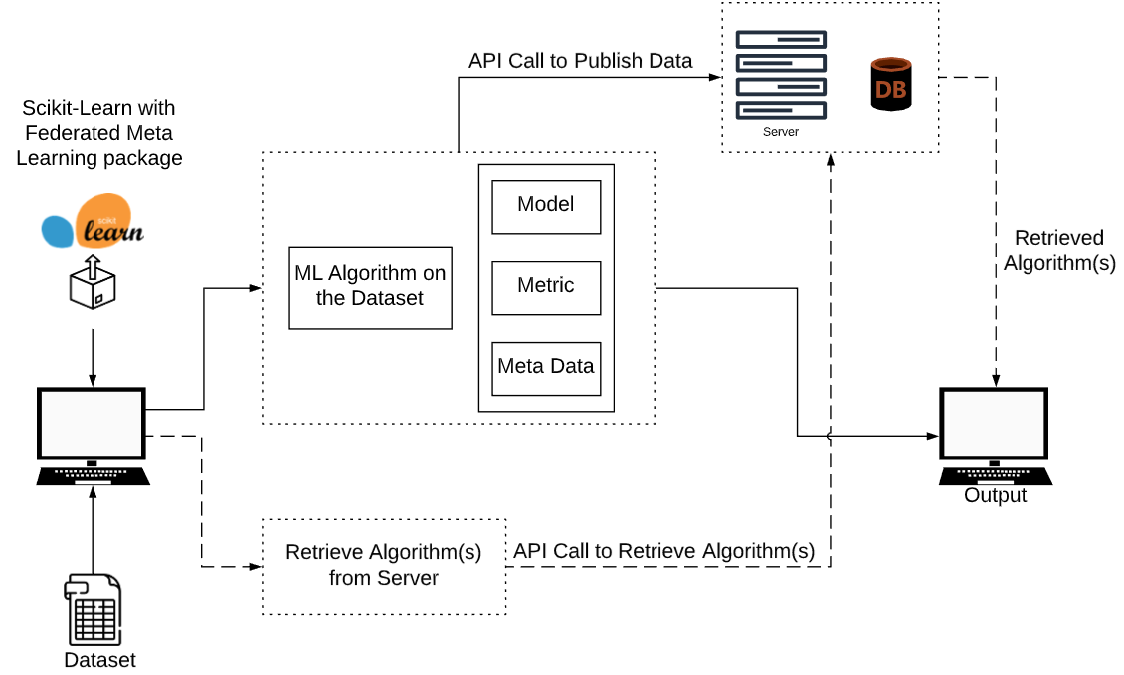
\includegraphics[width=3.5in]{architecture-diagram.PNG}
    \caption{Architecture Diagram}
    \label{architecture-diagram}
\end{figure}

The input to COOL-TOOL-NAME is the hashed dataset of the task, and the output is a recommendation for the potentially best performing algorithm(s) to solve that task (see Figure 1). This recommendation consists simply of a list of the best algorithms or simply a single best performing algorithm and their predicted performance values. In its simplest form, COOL-TOOL-NAME is a knowledge base or directory of algorithms-data performance measures. Here we want to introduce the concept called “Federated Meta-Learning” (FML), COOL-TOOL-NAME is an implementation of this concept. To the best of our knowledge this concept is novel. The term “Federated Meta Learning” has only been used once before by Chen et al. but in a different context [4]. This knowledge base is built and updated by users who use COOL-TOOL-NAME by sending their model’s and dataset’s meta-data via scikit-learn to the tool.




%% The file named.bst is a bibliography style file for BibTeX 0.99c
\bibliographystyle{named}
\bibliography{ijcai20}

\end{document}

